%%% Notice: This file contains a large number of \verb's 
%%%         or verbatim environments in order to display command names
%%%         or examples.  But the use of \verb/verbatim is *not* recommended. 
%%% ver.6 2015/01/05 
\documentclass{pasj01}
\usepackage{graphicx}

\draft 
\Received{$\langle$reception date$\rangle$}
\Accepted{$\langle$acception date$\rangle$}
\Published{$\langle$publication date$\rangle$}
%% \SetRunningHead{Astronomical Society of Japan}{Usage of \texttt{pasj00.cls}}

\begin{document}

\title{Photometric Classification of the HSC Transients through Machine Learning}
\author{PASJ Editorial Office}%
\altaffiltext{}{Astronomical Society of Japan, c/o National Astoronomical Observatory of Japan, 
 2-21-1 Osawa, Mitaka, Tokyo 181-8588, Japan }
\email{***@***.***.***}

\KeyWords{key word${}_1$ --- key word${}_2$ --- \dots --- key word${}_n$}

\maketitle

\begin{abstract}
abstract  
\end{abstract}

\section{Introduction : Suzuki}
\subsection{Increase in the number of discovered supernovae}
\begin{itemize}
\item DES, LSST
\item Necessity of machine learning
\end{itemize}
\subsection{Supernova survey}
\begin{itemize}
\item Past surveys
\item Subaru/HSC survey
\end{itemize}
\subsection{Supernovae type classification}
\begin{itemize}
\item SCP
\item SNPCC
\item PLAsTiCC
\end{itemize}
%
\section{Methods : Suzuki}
\subsection{Tasks in HSC survey}
\begin{itemize}
\item Classification of SN Ia
\item Observation schedule
\item Type classification before peak
\end{itemize}
\subsection{Classification methods in HSC survey}
%
\subsubsection{Creating simulated data}
\begin{itemize}
\item Used model and parameters
\item Type distribution
\item 
\end{itemize}
%
\subsubsection{Models : Imoto/Takahashi}
\begin{itemize}
\item DNN
\item Binary and Multi-type
\end{itemize}
%
%
\section{Validation with simulated data}
\subsection{Sim. data (SNANA)}
\begin{itemize}
\item Flow of simulated data classification
\item Distribution of predictions in redshift (figure)
\item ROC curves (figure) and AUCs
\end{itemize}
%
\subsection{PLAsTiCC data (or SNPCC)}
\begin{itemize}
\item Validation using a part of samples with answers
\item Comparison with the 1st model in PLAsTiCC (If possible)
\item 
\end{itemize}
%
\section{Application to HSC survey}
\begin{itemize}
\item Observation schedule
\item Classifications were updated as observations progress
\item Using 15 to 20 data points for each classification
\end{itemize}
%
\subsection{Real time classification (Binary)}
\begin{itemize}
\item Classification examples (figure)
\item Performance in the survey
\item Follow-up Observation
\end{itemize}
%
\begin{figure}[ht]
  \begin{center}
     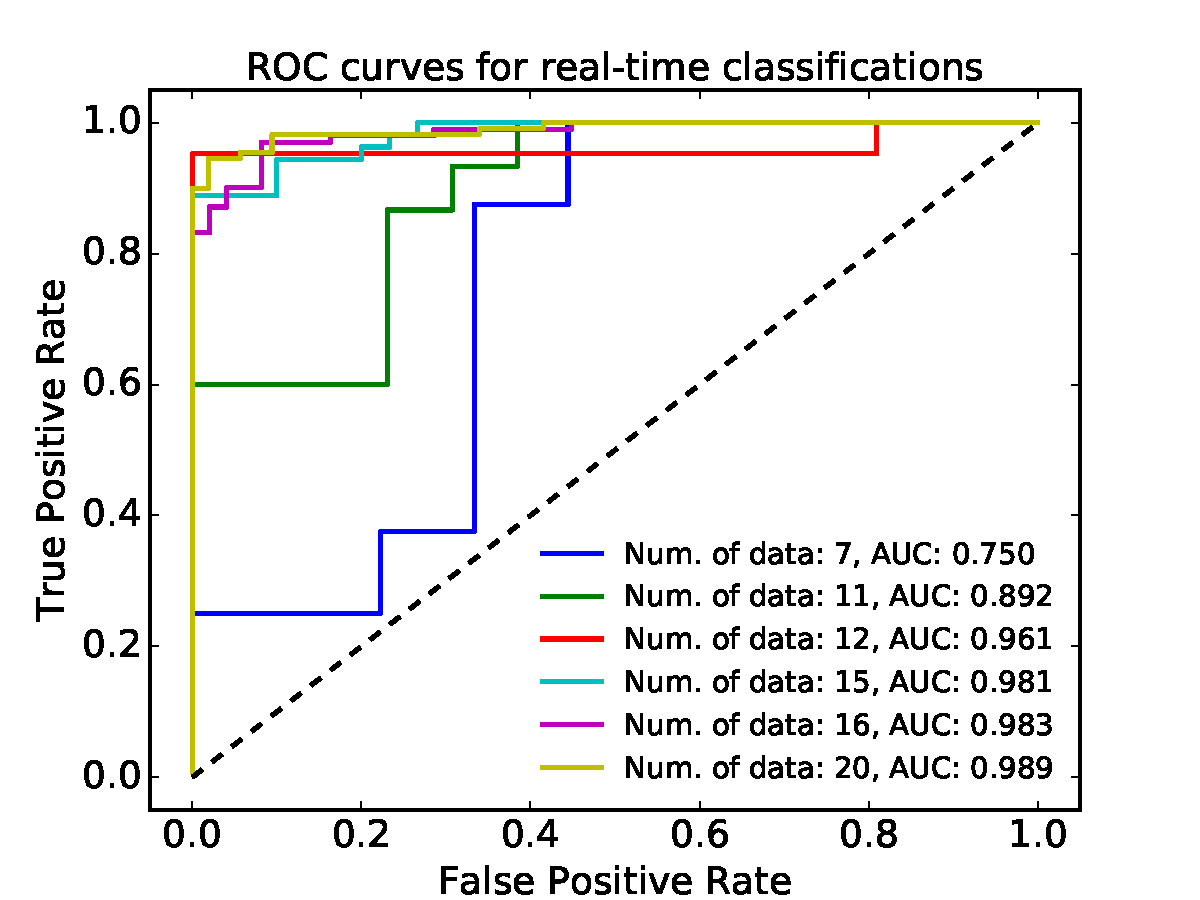
\includegraphics[width=\columnwidth]{figures/Realtime_ROCs.eps}
  \end{center}
  \caption{%
  ROC curves for real-time data
  }%
  \label{fig:realtimeROCs}
\end{figure}
%
%
\begin{figure}[ht]
  \begin{center}
     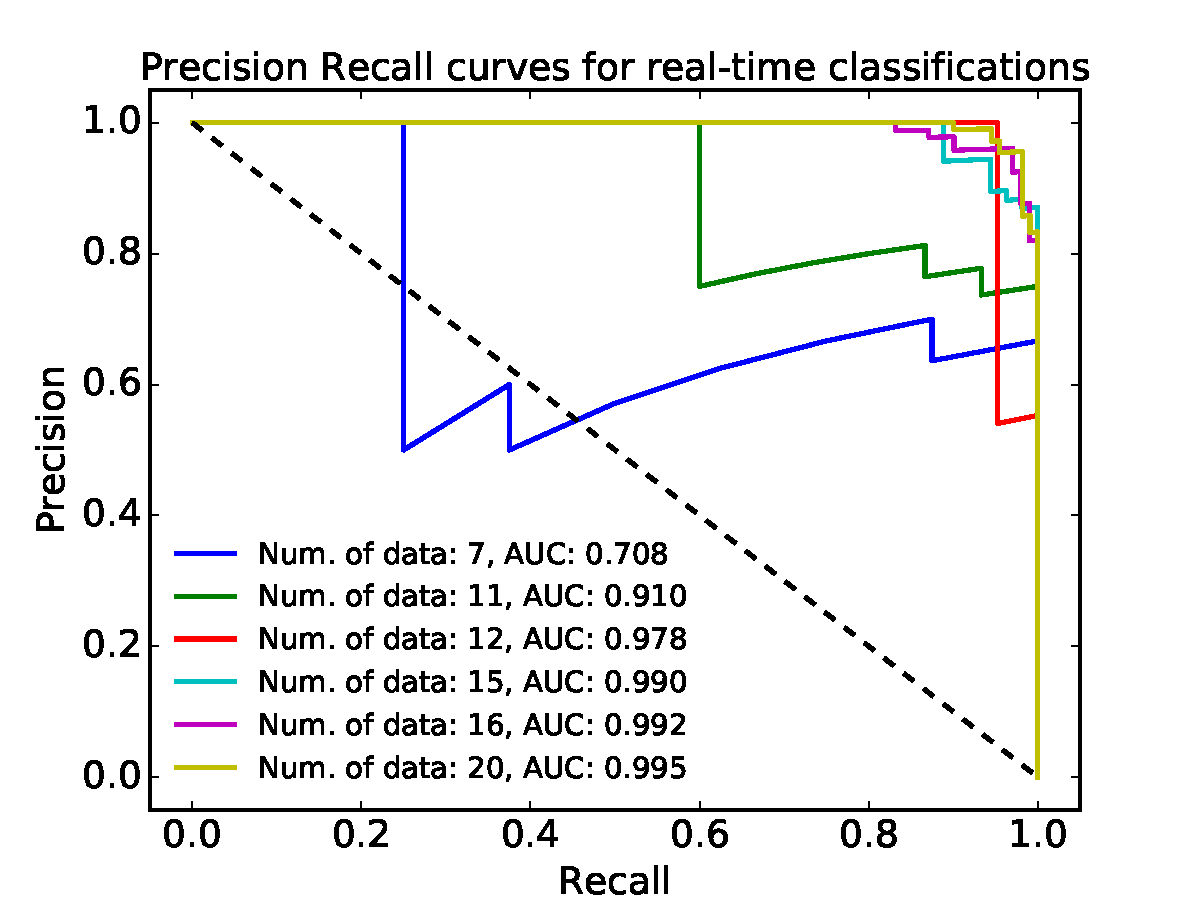
\includegraphics[width=\columnwidth]{figures/Realtime_PreRecs.eps}
  \end{center}
  \caption{%
  Precision Recall curves for real-time data
  }%
  \label{fig:realtimePreRecs}
\end{figure}
%
%
\begin{figure}[ht]
  \begin{center}
     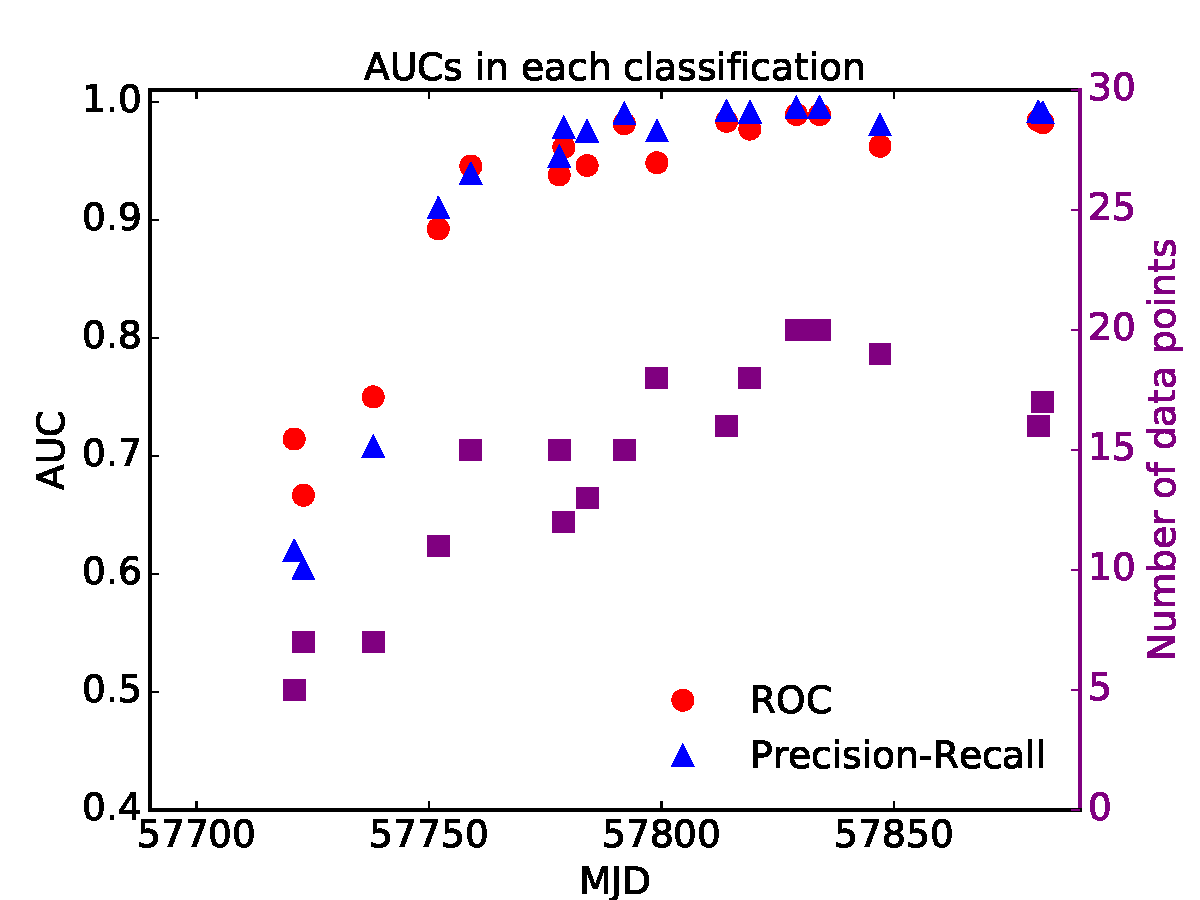
\includegraphics[width=\columnwidth]{figures/AUCs_190215.eps}
  \end{center}
  \caption{%
  Performance in the survey
  }%
  \label{fig:realtimeAUCs}
\end{figure}
%
\subsection{Full data classification (Binary and Multi)}
\begin{itemize}
\item DPP and SNP
\item Binary classification
\item Multi-type classification
\item Comparison with other classification results (template fit, chi2 fit, PLAsTiCC 1st (If possible))
\item 
\end{itemize}

%
\begin{figure}[ht]
  \begin{center}
     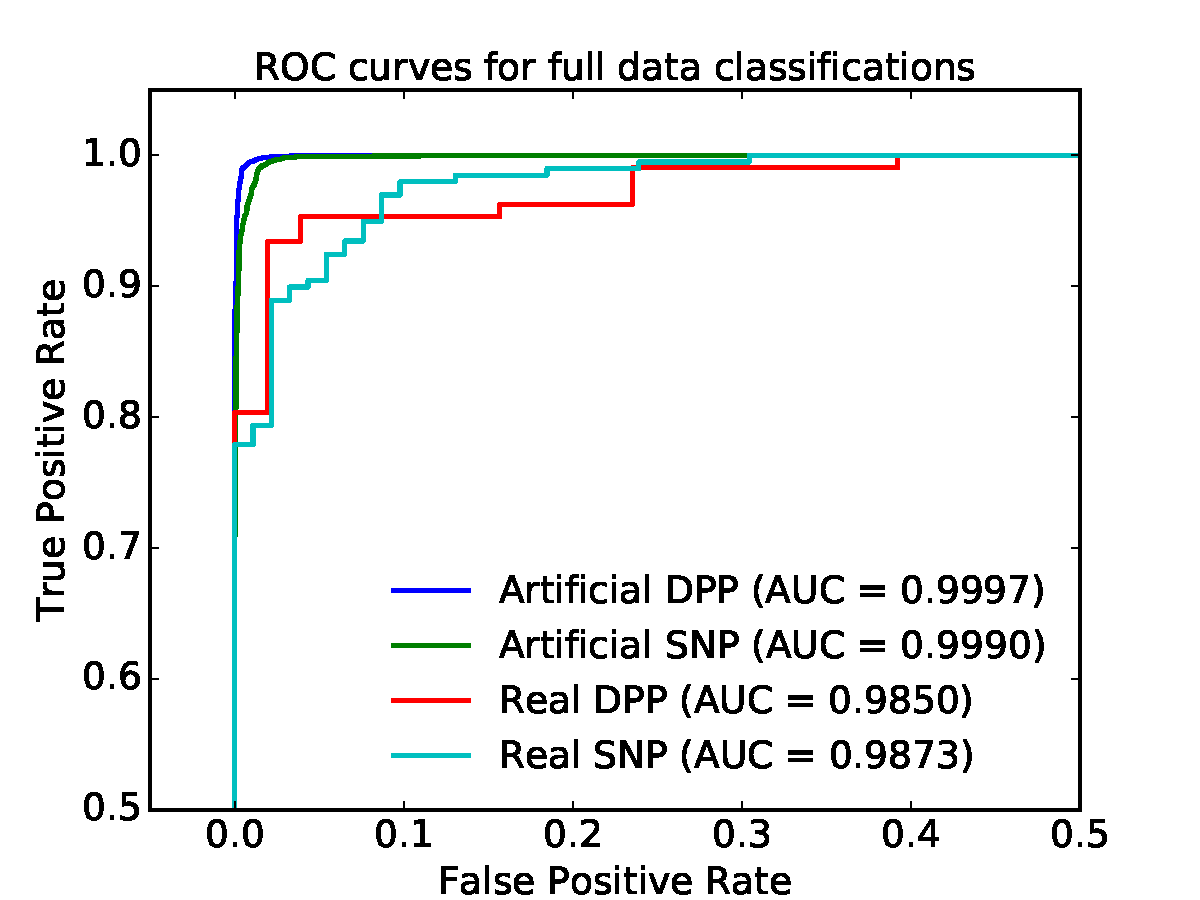
\includegraphics[width=\columnwidth]{figures/Fulldata_ROC.eps}
  \end{center}
  \caption{%
  ROC curves for full data
  }%
  \label{fig:fullROC}
\end{figure}
%
%
\begin{figure}[ht]
  \begin{center}
     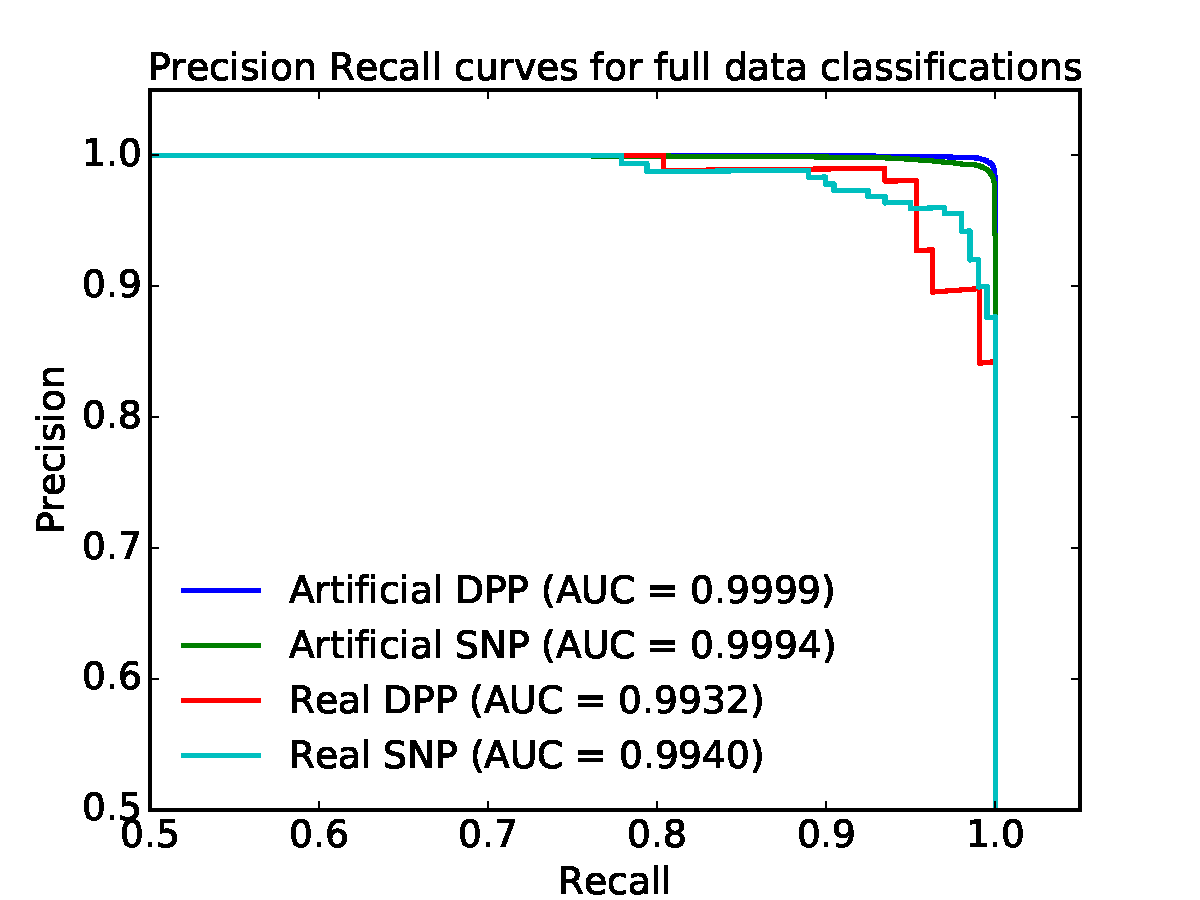
\includegraphics[width=\columnwidth]{figures/Fulldata_PreRec.eps}
  \end{center}
  \caption{%
  Precision Recall curves for full data
  }%
  \label{fig:fullPreRec}
\end{figure}
%

\begin{table}[ht]
\tbl{Confusion matrix for artificial data(full data, DPP)}{
\begin{tabular}{llrrrrrrr}
\hline
\multicolumn{2}{l}{accuracy: 0.987} & \multicolumn{5}{l}{Predicted} & \multicolumn{1}{l}{Sum} & \multicolumn{1}{l}{Recall} \\ \cline{3-7}
\multicolumn{2}{l}{} & \multicolumn{1}{l}{Ia} & \multicolumn{1}{l}{Ibc} & \multicolumn{1}{l}{IIL} & \multicolumn{1}{l}{IIn} & \multicolumn{1}{l}{IIP} & \multicolumn{1}{l}{} & \multicolumn{1}{l}{} \\ \hline
Actual & Ia & 11480 & 1 & 0 & 0 & 3 & 11484 & 1.000 \\ \cline{2-9} 
& Ibc & 76    & 1070 & 0  & 4   & 69   & 1219  & 0.878 \\ \cline{2-9} 
& IIL & 3     & 3    & 42 & 2   & 4    & 54    & 0.778 \\ \cline{2-9} 
& IIn & 0     & 1    & 0  & 552 & 0    & 553   & 0.998 \\ \cline{2-9} 
& IIP & 37    & 5    & 0  & 4   & 3246 & 3292  & 0.986 \\ \hline
\multicolumn{2}{l}{Sum} & 11596 & 1080 & 42 & 562 & 3322 & 16602 &       \\ \hline
\multicolumn{2}{l}{Precision} & 0.990 & 0.991 & 1.000 & 0.982 & 0.977 & & \\ \hline
\end{tabular}}\label{tab:fullCMDPP}
\end{table}
%
\begin{table}[ht]
\tbl{Confusion matrix for artificial data(full data, SNP)}{
\begin{tabular}{llrrrrrrr}
\hline
\multicolumn{2}{l}{accuracy: 0.956} & \multicolumn{5}{l}{Predicted} & \multicolumn{1}{l}{Sum} & \multicolumn{1}{l}{Recall} \\ \cline{3-7}
\multicolumn{2}{l}{} & \multicolumn{1}{l}{Ia} & \multicolumn{1}{l}{Ibc} & \multicolumn{1}{l}{IIL} & \multicolumn{1}{l}{IIn} & \multicolumn{1}{l}{IIP} & \multicolumn{1}{l}{} & \multicolumn{1}{l}{} \\ \hline
Actual & Ia & 9318 & 4 &0 & 1 &12 & 9335 & 0.998 \\ \cline{2-9} 
& Ibc & 151    & 733 & 0  & 12   & 272   & 1168  & 0.628 \\ \cline{2-9} 
& IIL & 6     & 2    & 19 & 1   & 29    & 57    & 0.333 \\ \cline{2-9} 
& IIn & 0     & 1    & 0  & 494 & 35    & 530   & 0.932 \\ \cline{2-9} 
& IIP & 77    & 9    & 0  & 9   & 3052 & 3147  & 0.970 \\ \hline
\multicolumn{2}{l}{Sum} & 9552 & 749 & 19 & 517 & 3400 & 14237 &       \\ \hline
\multicolumn{2}{l}{Precision} & 0.976 & 0.979 & 1.000 & 0.956 & 0.898 & & \\ \hline
\end{tabular}}\label{tab:fullCMSNP}
\end{table}
%
\section{Conclusion}
\begin{itemize}
\item 
\item 
\item our new method(2DGP+LGBM)
\end{itemize}

\begin{ack}
 a brief note for an acknowledgment, if any.   
\end{ack}



\end{document}